\section{落下手法の変化}

本文中における実験は,電磁石ホルダーを用いて鋼球を把持しているため,強磁性の材質の物体のみ把持することができる.
他の物質の物体を把持することのできる爪式ピッキングツールを用いて物体の把持を行い,球の落下試験を行った.
以下にその方法と結果を示す.

\subsection{実験方法}

今回,落下球の把持の方法を変化させただけであるので,実験装置の落下球把持の部分以外は先述の方法と同一である.

\subsubsection{実験装置}

実験装置の模式図をFig.\ref{fig:device2}に示す.先述の通り,電磁石ホルダーではなく,爪式ピックアップツールを用いて球の把持を行った.そして,ピックアップツールの開放を行うことで球を落下させた.それ以外に関しては,本文中の実験装置と同一である.

\begin{figure}[h]
    \centering
    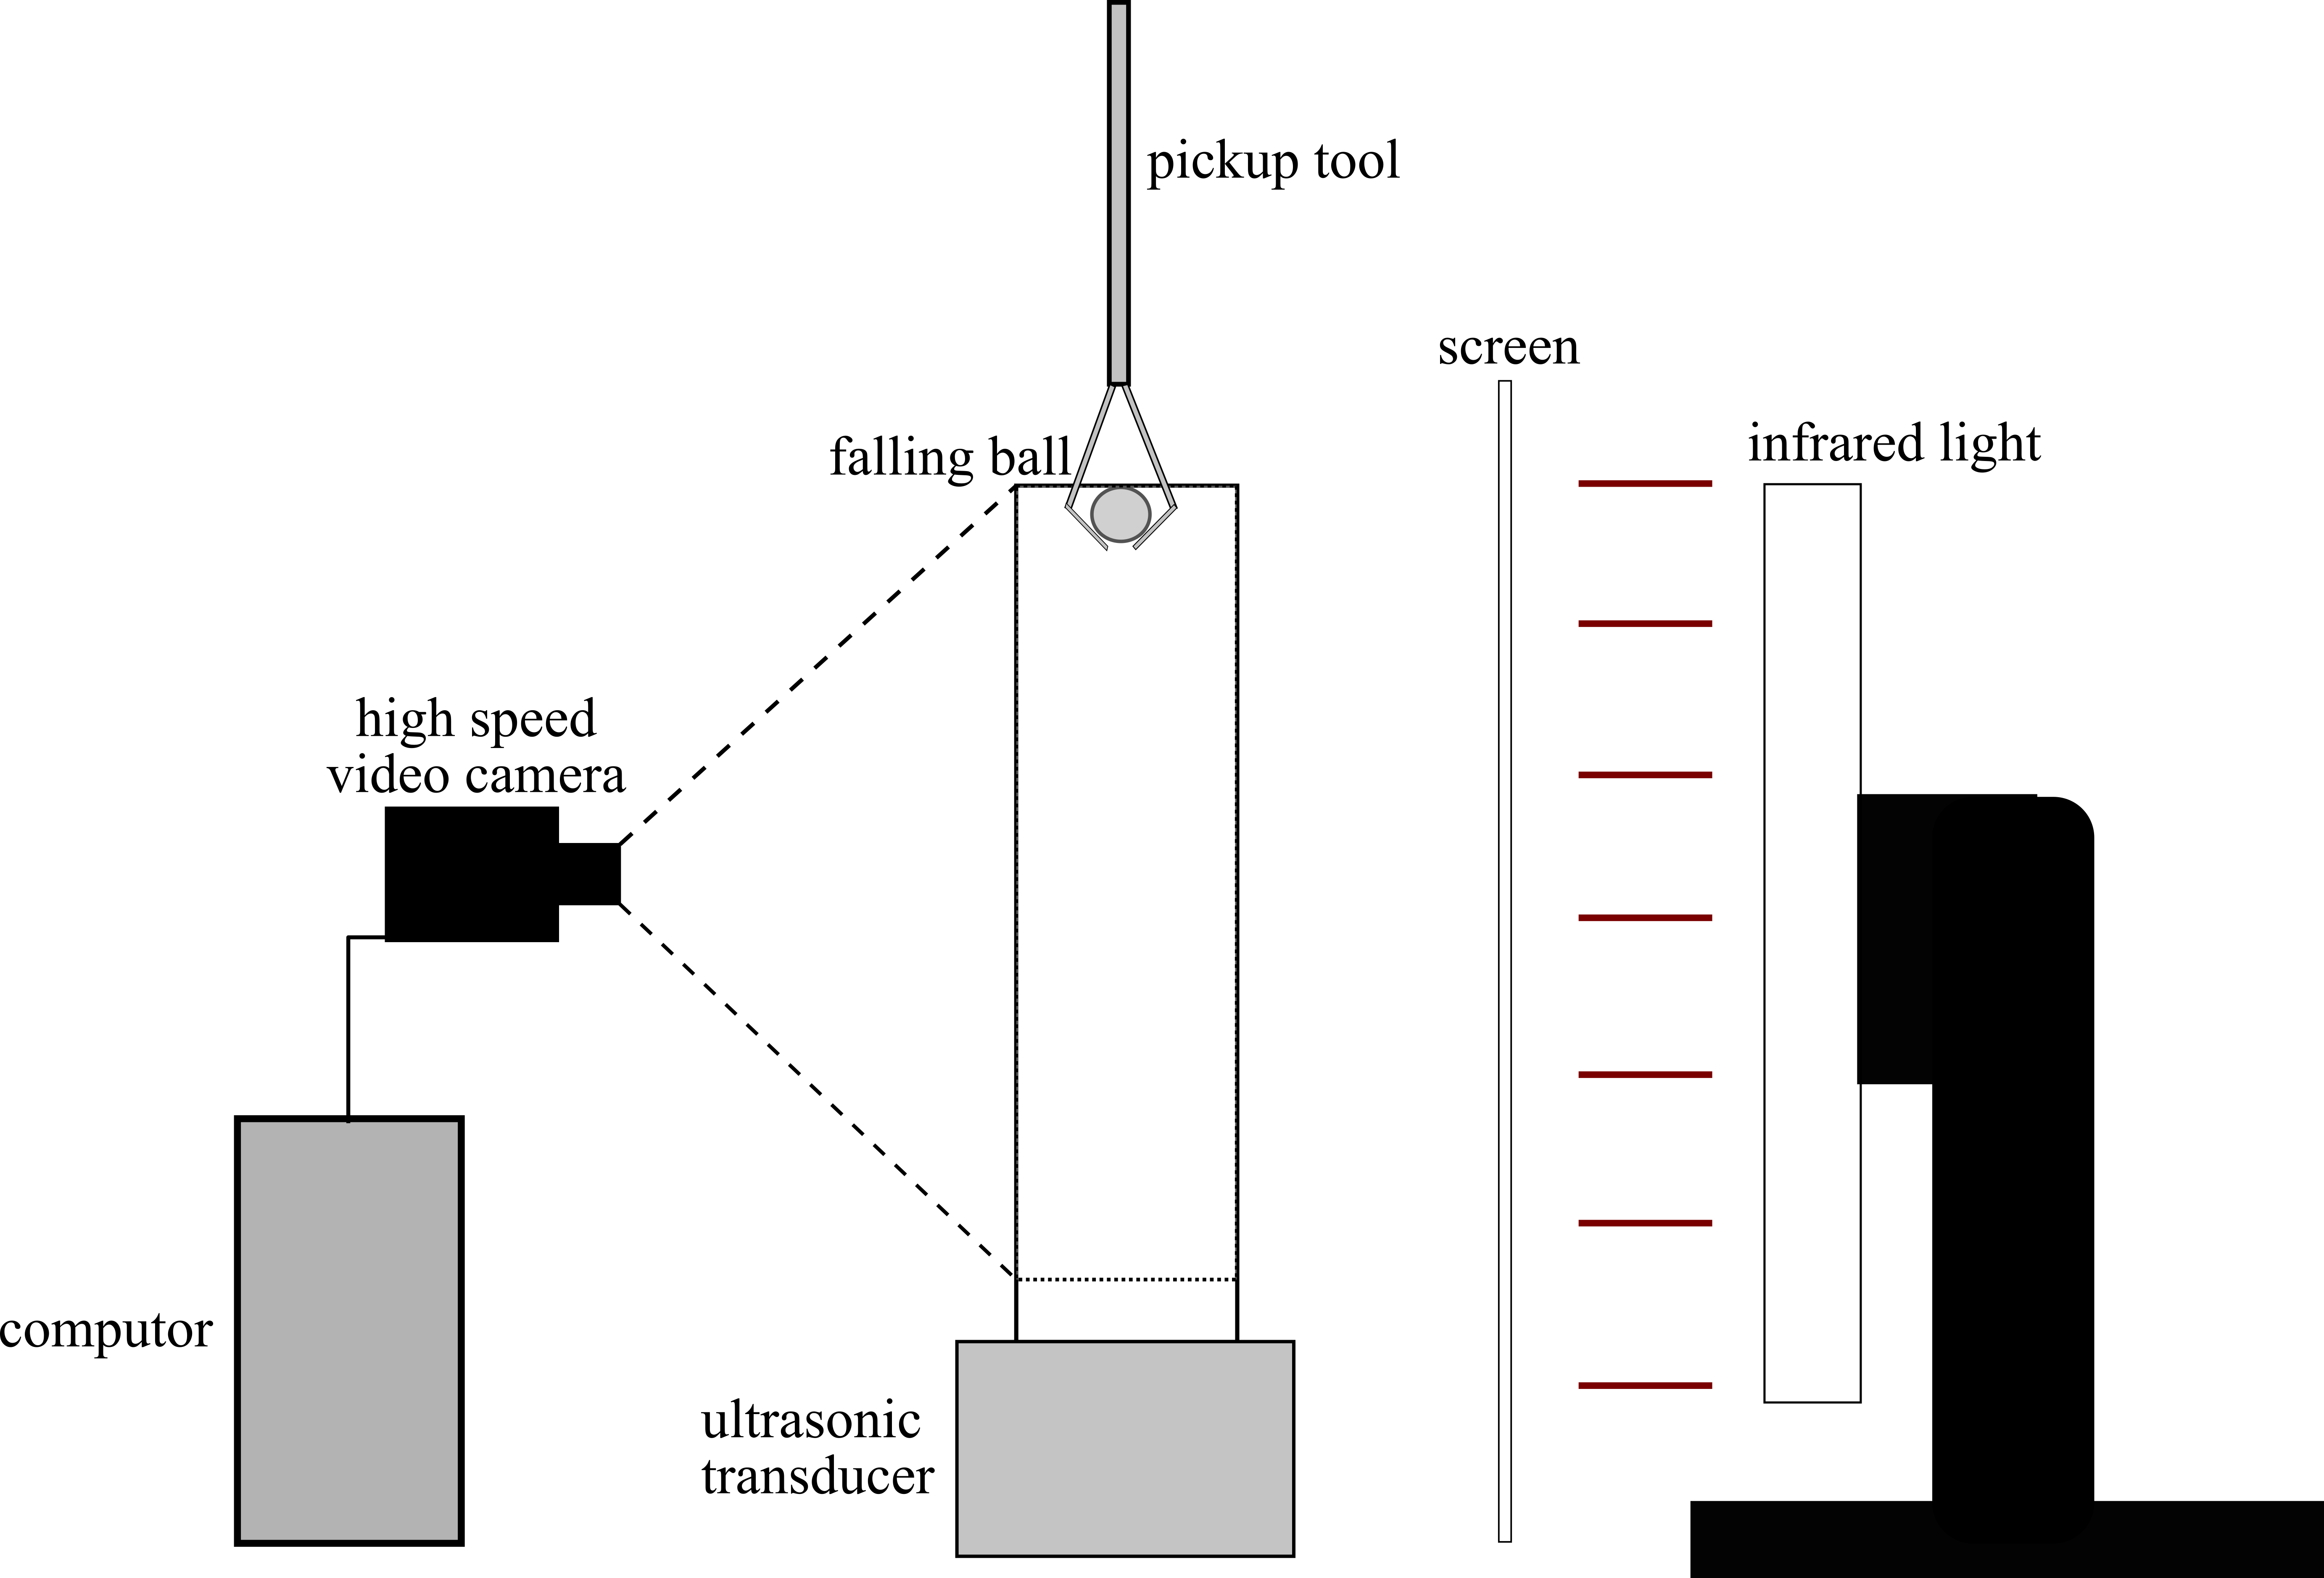
\includegraphics[clip,width=12.0cm]{X-Appendix/device.png}
    \caption{Schematic view of the experimental apparatus.}
    \label{fig:device2}
\end{figure}

\subsection{落下球 実験結果}

1wt.\%PAA溶液中における球の落下速度を解析した結果をFig.\ref{fig:1-1PAA-falling}に示す.縦軸は落下速度,横軸は落下開始時からの経過時間である.先述の電磁石ホルダを用いたFig.\ref{fig:1PAA-falling}とは異なり,超音波照射の有無において落下速度の高速化は見られなかった.一方で,先行研究であるIwamuro {\it et al.}\cite{ref:9}と同様に初めの加速後は減速し一定速度となった.

また,電磁石ホルダを用いた場合と同様に,超音波照射なしの状態における1から5試行目の結果をFig.\ref{fig:1-1PAA-falling1-5}に,6から10試行目の結果をFig.\ref{fig:1-1PAA-falling6-10}に示す.また,超音波照射ありの状態における1から5試行目の結果をFig.\ref{fig:1-1onPAA-falling1-5}に,6から10試行目の結果をFig.\ref{fig:1-1onPAA-falling6-10}に示す.これら試行ごとの結果において,先述のFig.\ref{fig:1PAA-falling1-5}-\ref{fig:1onPAA-falling6-10}の結果とは異なり落下速度のばらつきが非常に小さくなっていた.

\begin{figure}[ht]
    \centering
    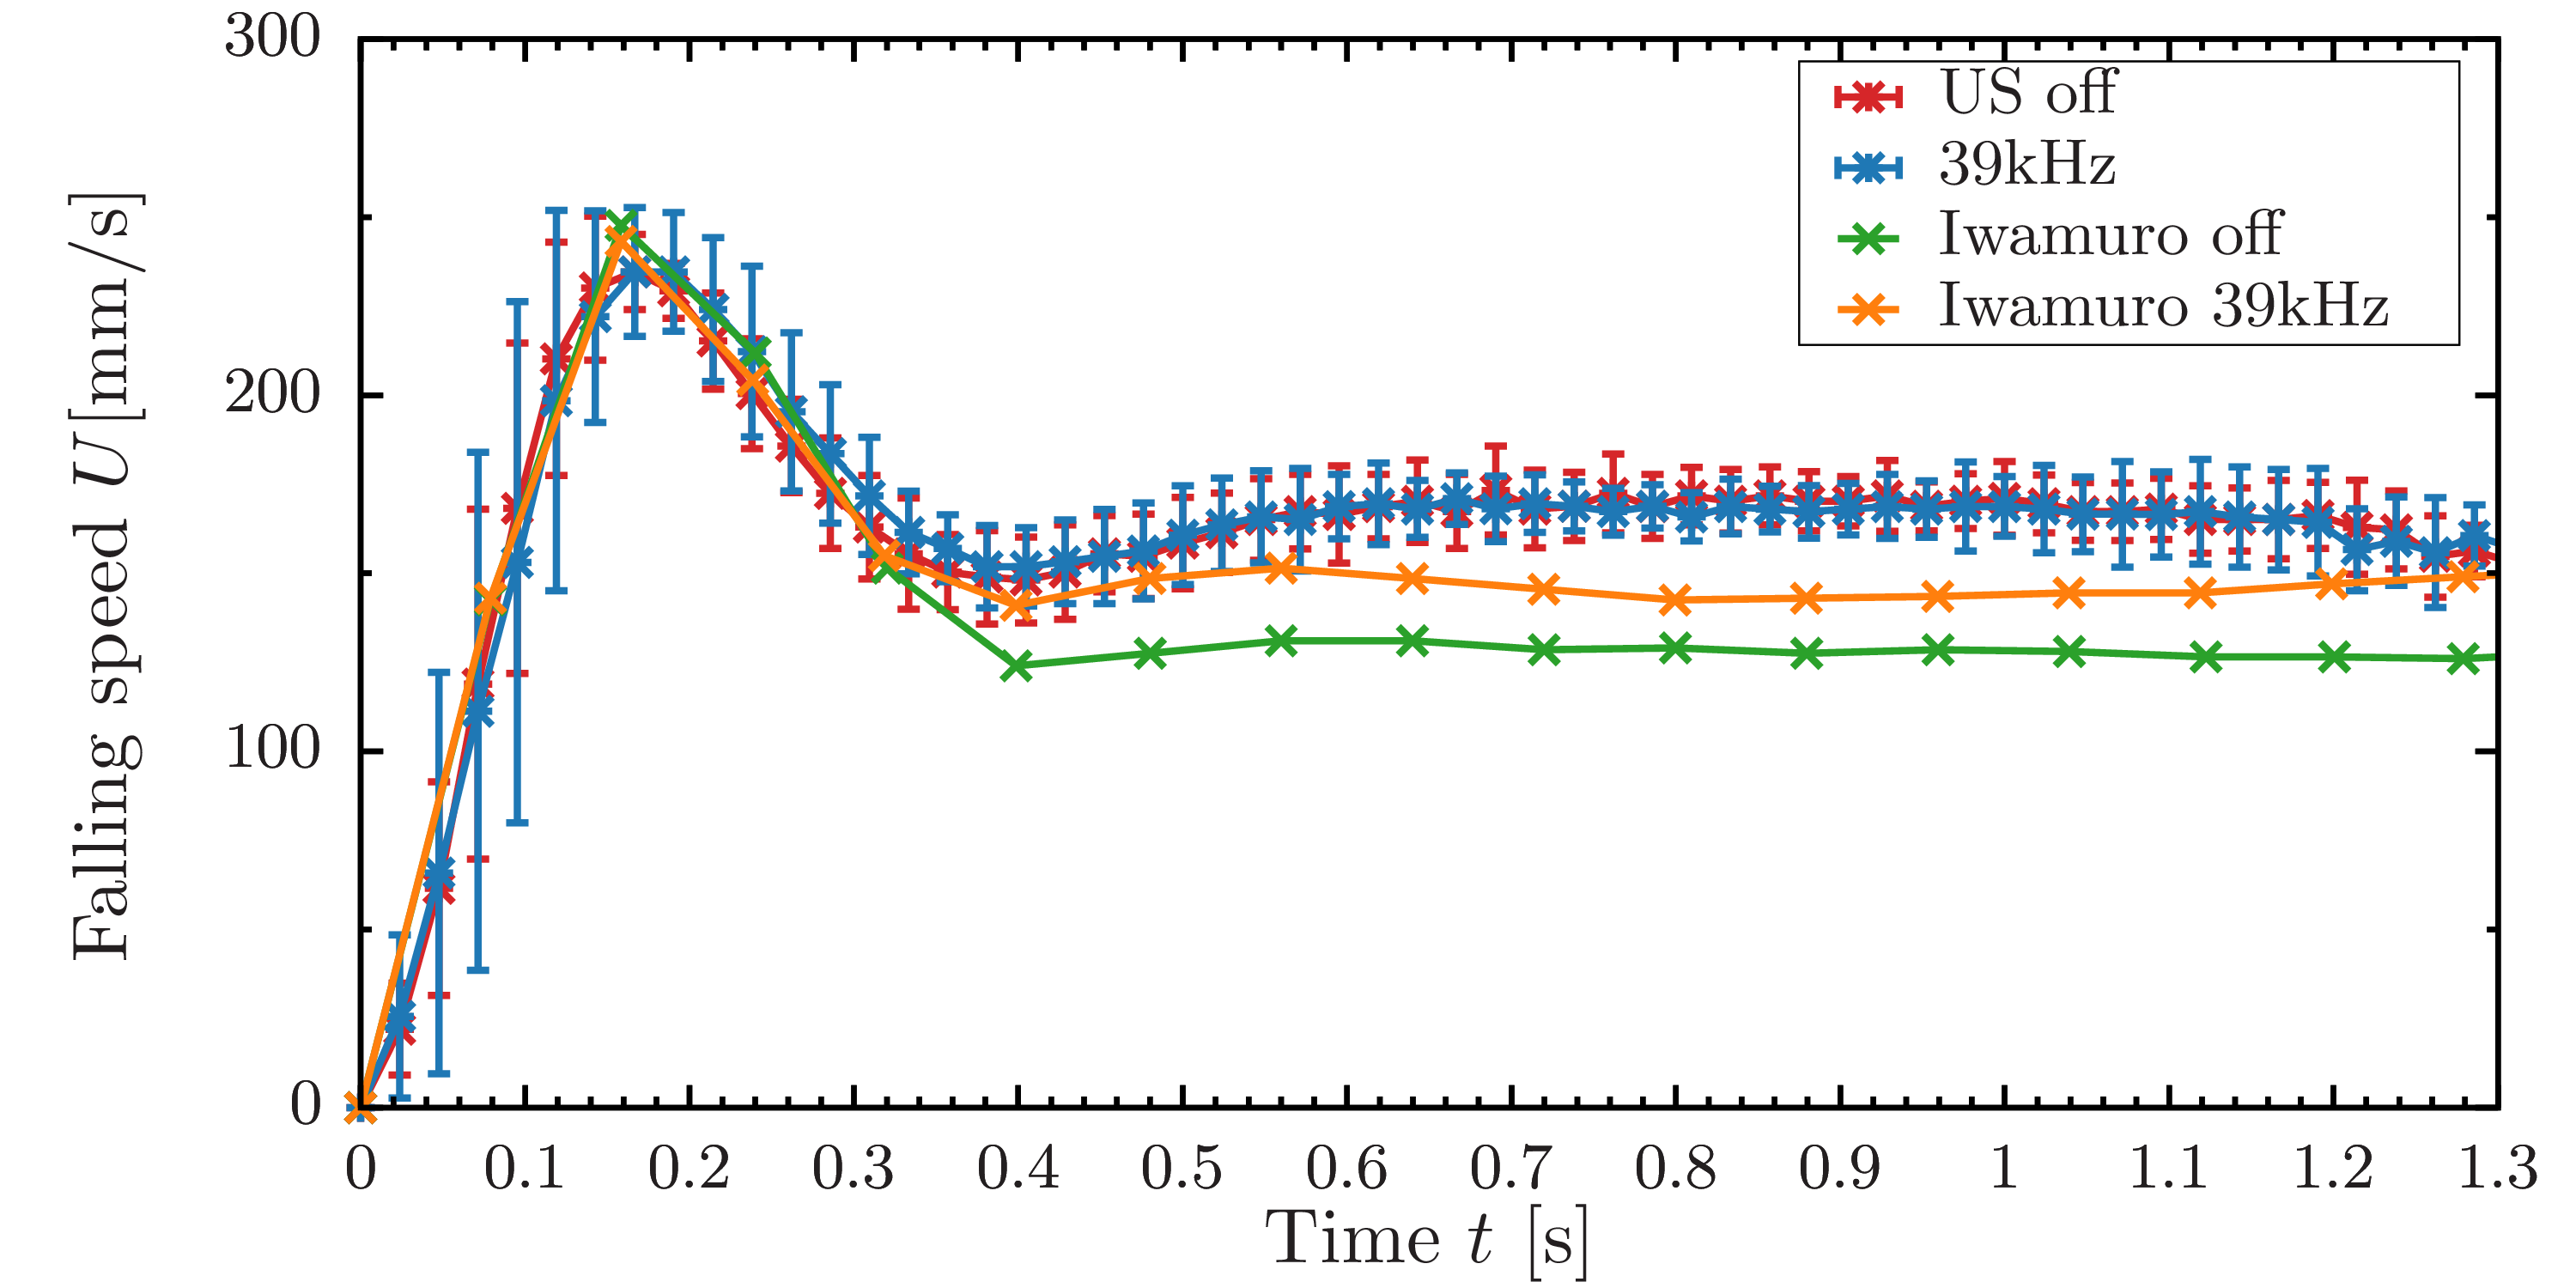
\includegraphics[width=12cm,clip]{./X-Appendix/s1.png}
    \caption{Falling velocity of a sphere in 1wt.\%PAA solution with and without ultrasound irradiation.}
    \label{fig:1-1PAA-falling}
    \centering
    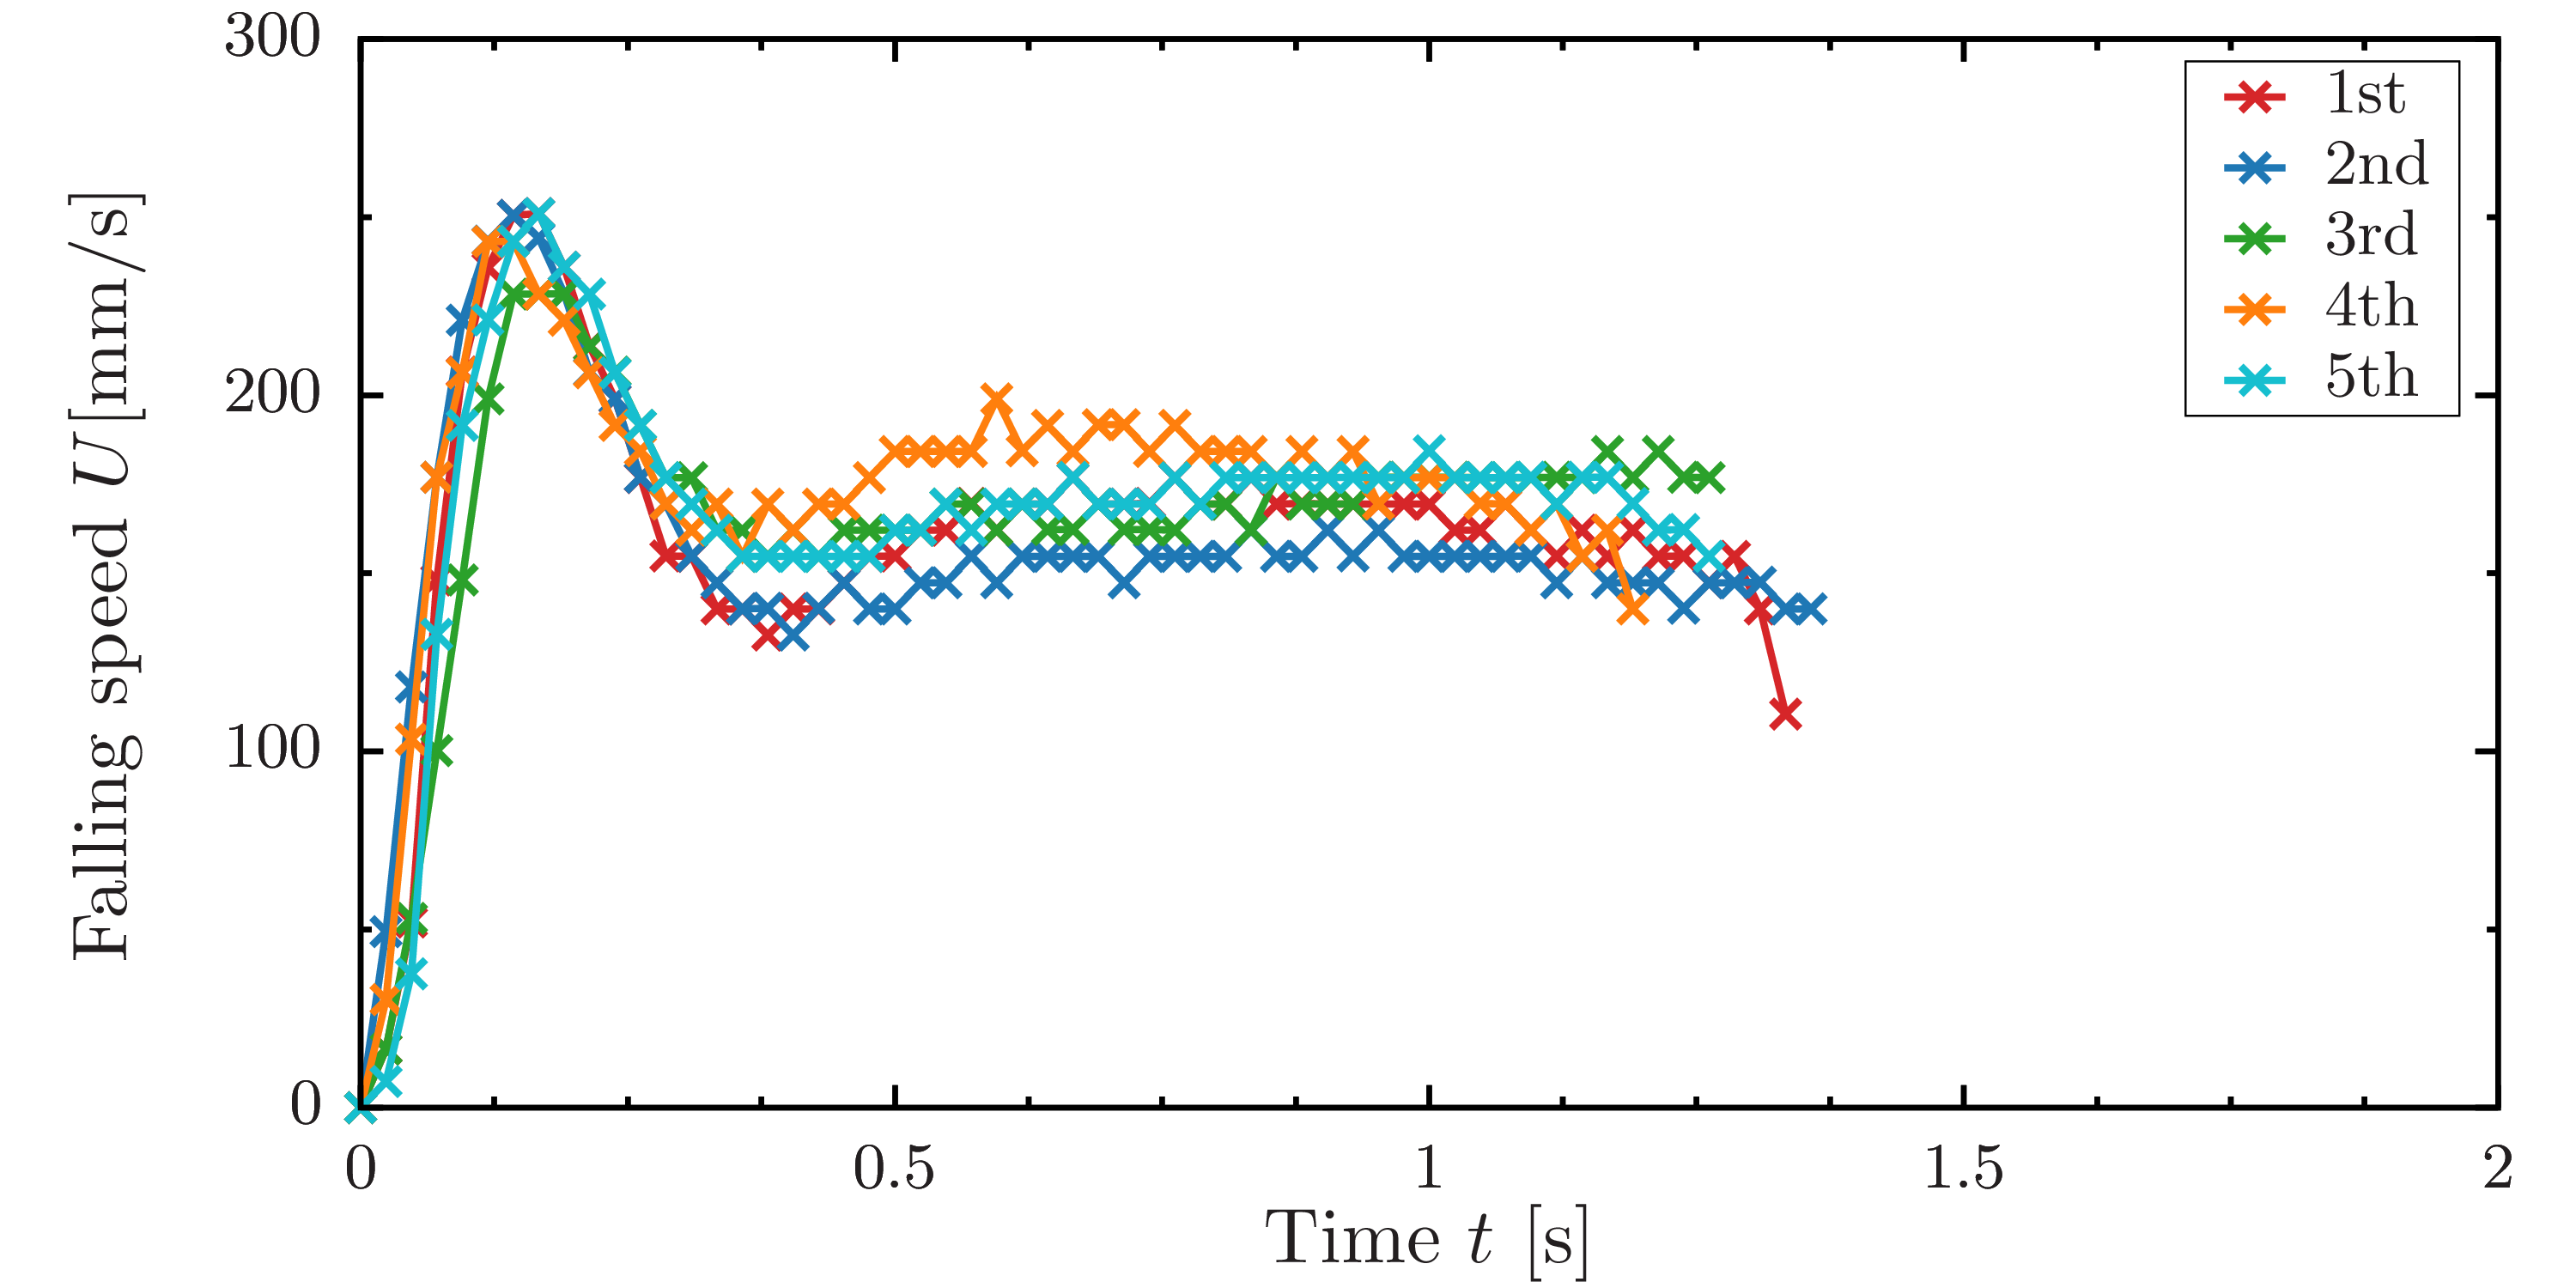
\includegraphics[width=12cm,clip]{X-Appendix/s1-0-1-5.png}
    \caption{Falling velocity of the sphere for each trial (\#1 to \#5) in 1wt.\%PAA solution without ultrasonic irradiation.}
    \label{fig:1-1PAA-falling1-5}
\end{figure}
\begin{figure}[ht]
    \centering
    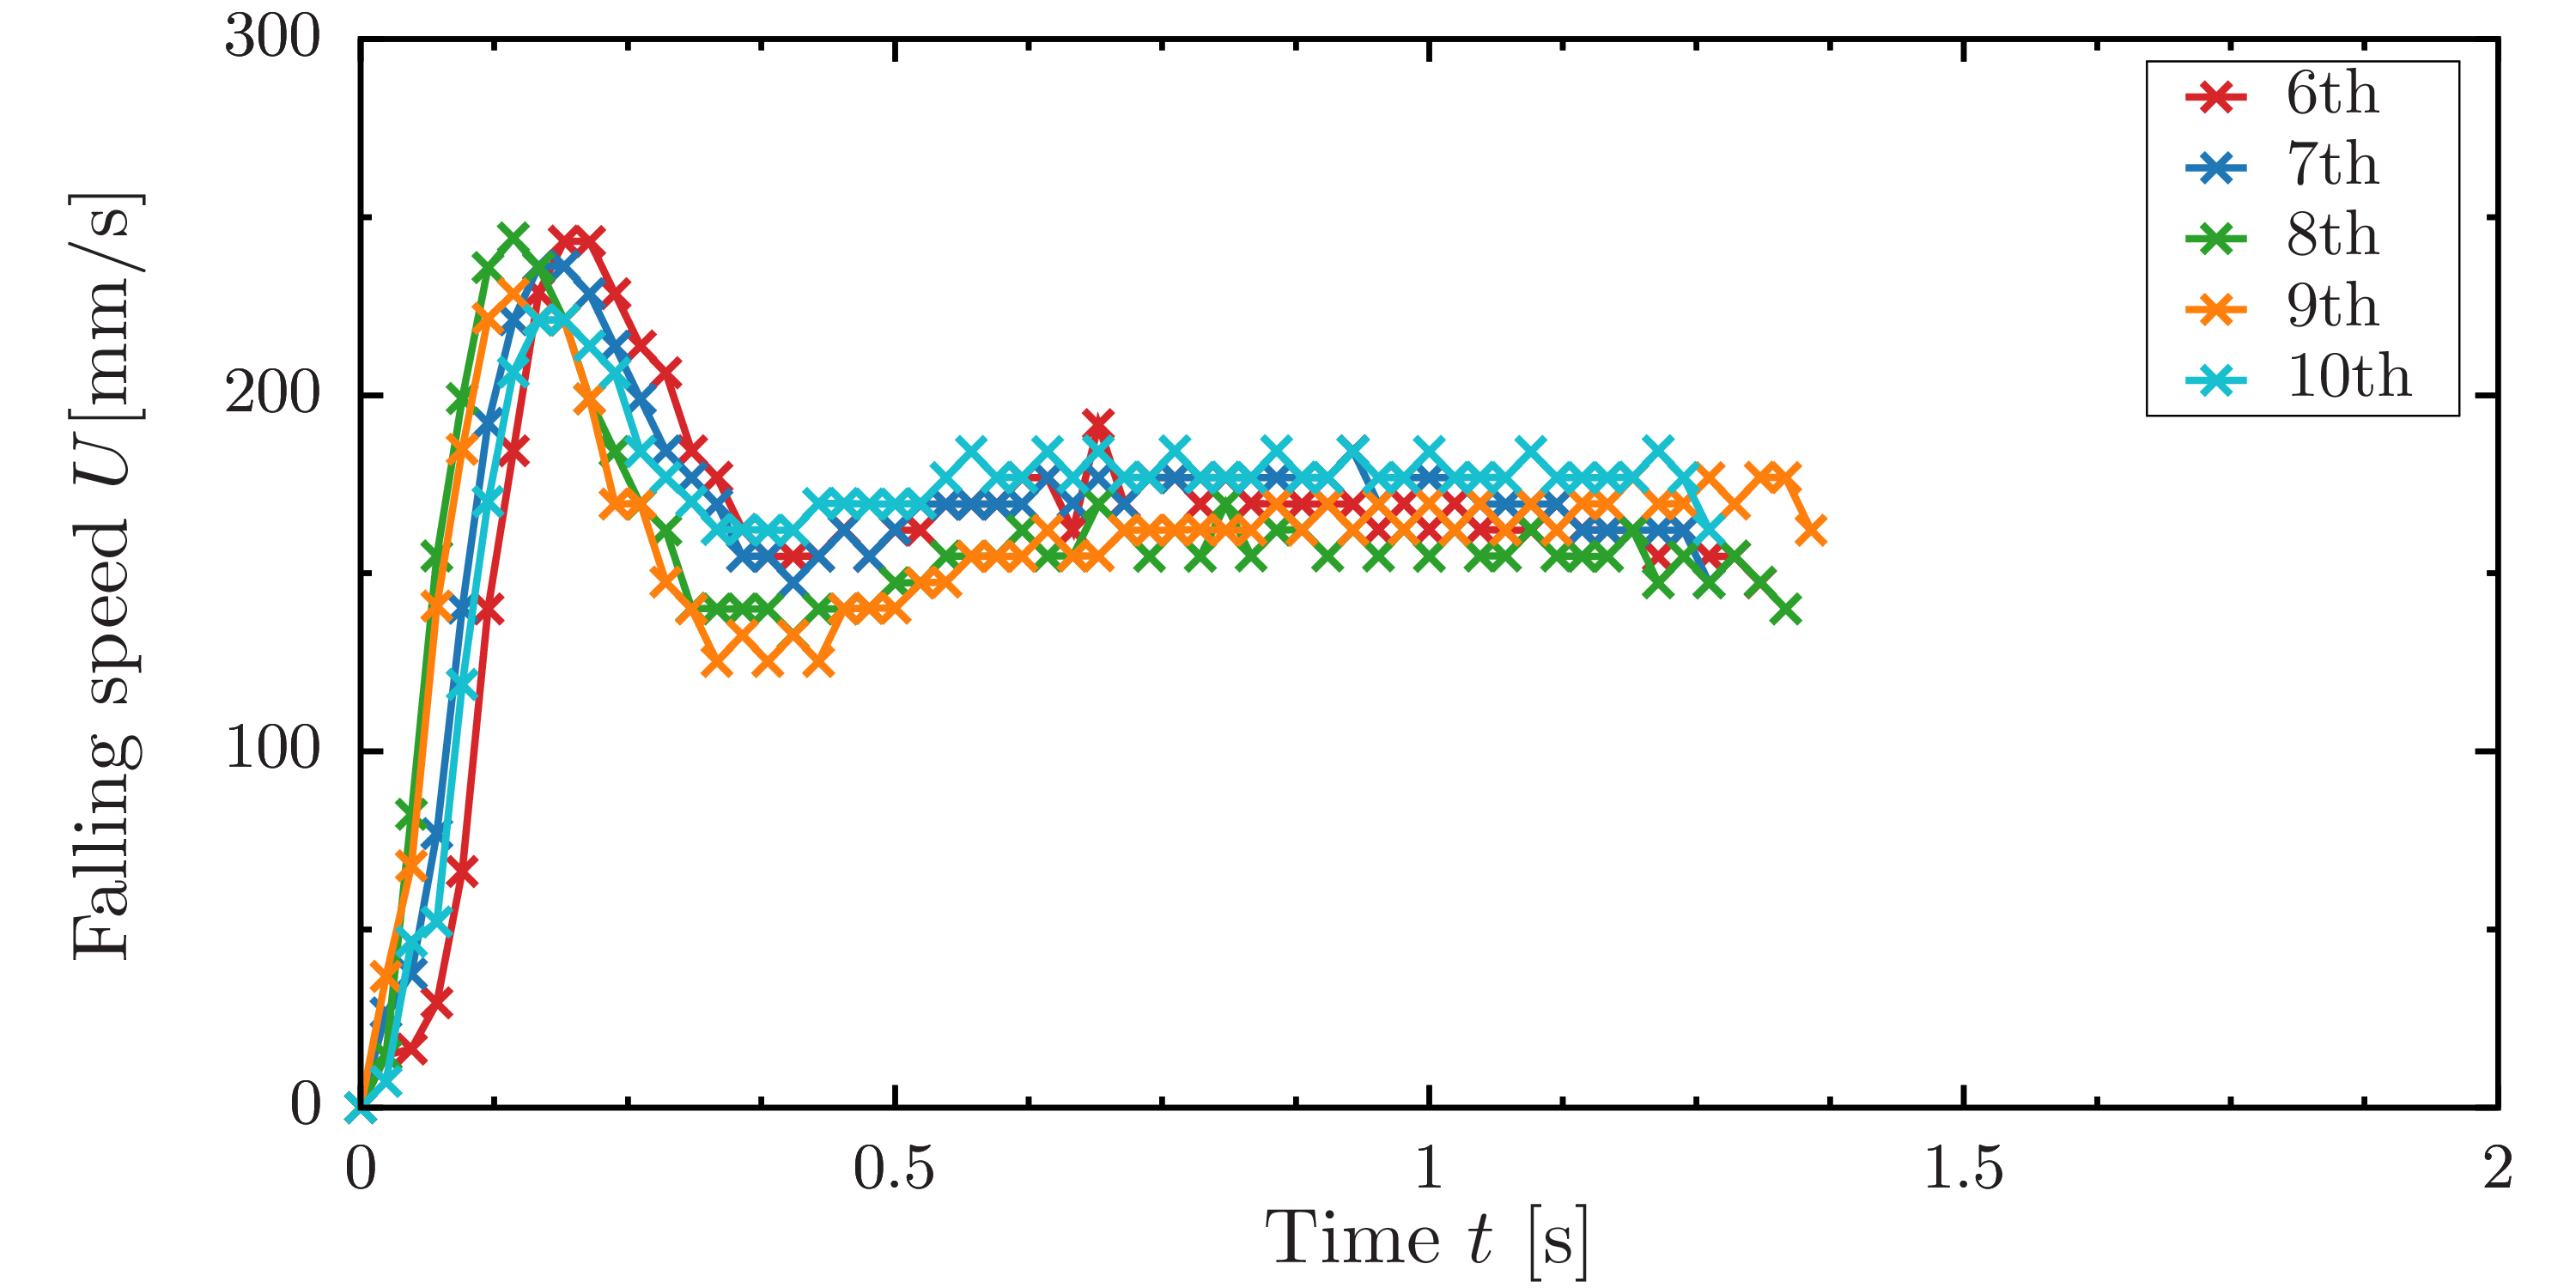
\includegraphics[width=12cm,clip]{X-Appendix/s1-0-6-10.png}
    \caption{Falling velocity of the sphere for each trial (\#6 to \#10) in 1wt.\%PAA solution without ultrasonic irradiation.}
    \label{fig:1-1PAA-falling6-10}
    \centering
    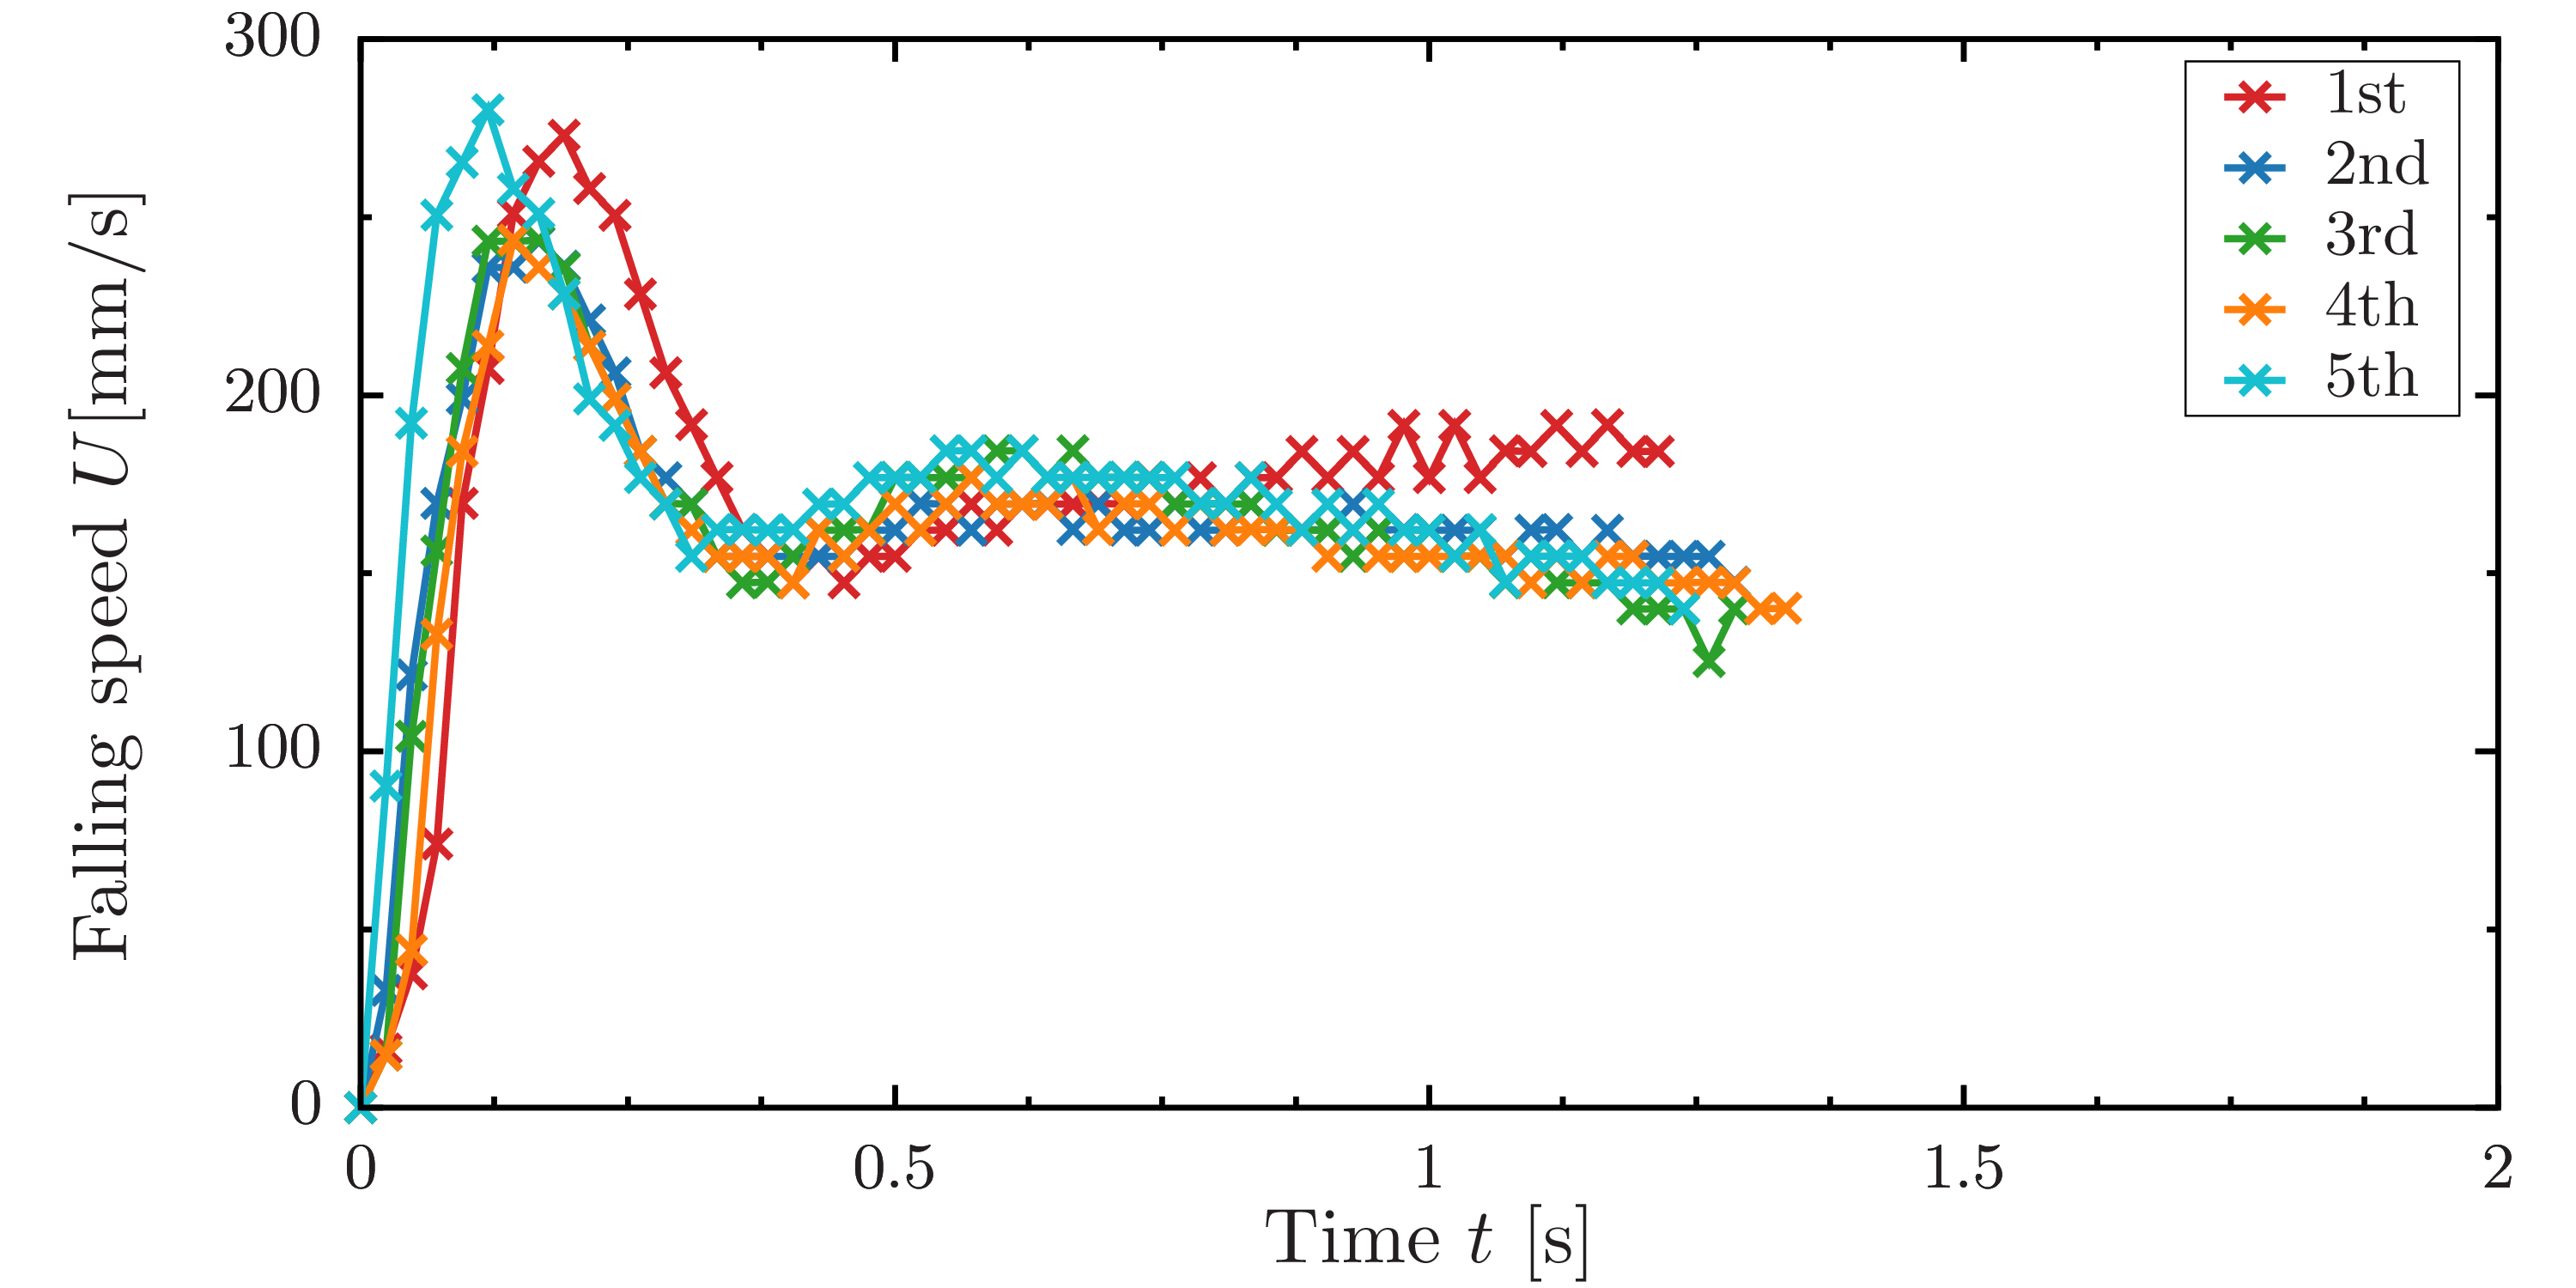
\includegraphics[width=12cm,clip]{X-Appendix/s1-39-1-5.png}
    \caption{Falling velocity of the sphere for each trial (\#1 to \#5) in 1wt.\%PAA solution with ultrasonic irradiation.}
    \label{fig:1-1onPAA-falling1-5}
    \centering
    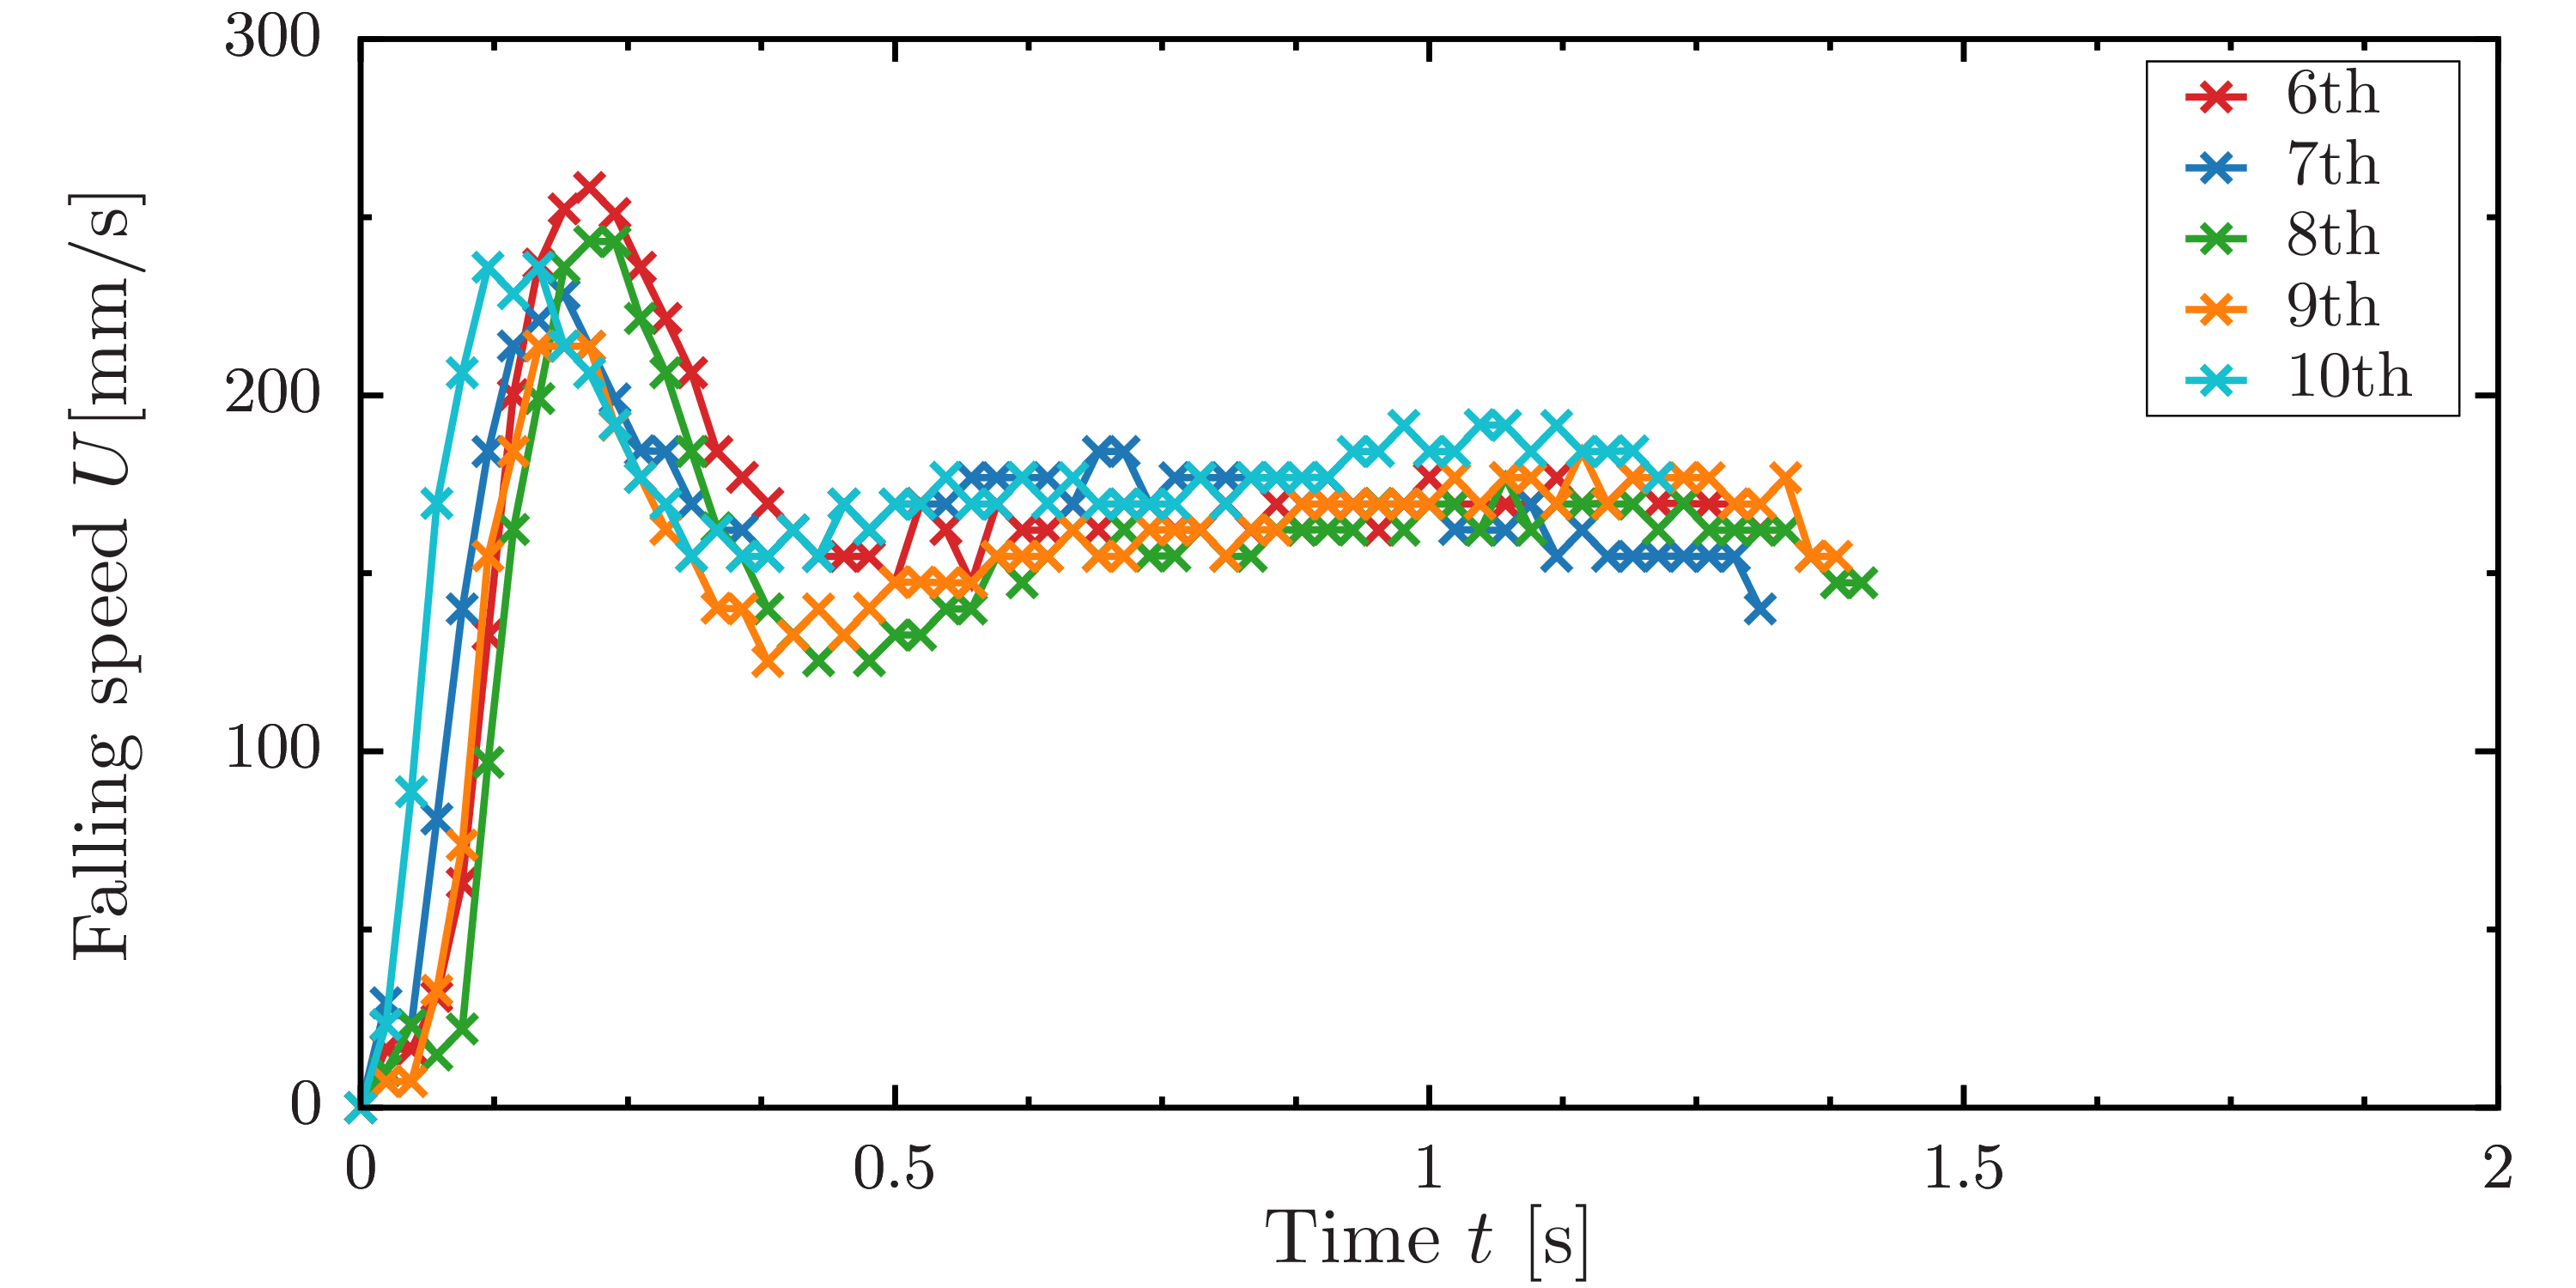
\includegraphics[width=12cm,clip]{X-Appendix/s1-39-6-10.png}
    \caption{Falling velocity of the sphere for each trial (\#6 to \#10) in 1wt.\%PAA solution with ultrasonic irradiation.}
    \label{fig:1-1onPAA-falling6-10}
\end{figure}

\subsection{考察}

電磁石ホルダを用いた把持方法と爪式ピッキングツールを用いた把持方法では試行ごとの落下速度の時間変化や超音波照射による高速化の有無において変化が見られた.以下に把持方法の変化による影響に関して検討を行う.

まず,電磁石ホルダを使用する場合,落下開始1分前に電源を切り,電磁石ホルダの把持力をゼロにする.しかし,落下させる対象の鋼球や溶液中に把持しているために存在する鋼製棒に磁性が残っている.また,落下球はPAA溶液中に存在するため浮力や粘弾性の影響を受ける.そのため落下開始時まで,把持している鋼製棒に接触したままとなっている.ここに,非常に弱い撃力を指で与え,落下させている.撃力による初速への影響
弾性によって減速が大きくなる可能性が存在する.

続いて,ピッキングツールを使用する場合に関して検討を行う.ピッキングホルダは球の把持を行っている爪を開くことによって,落下球の把持を開放し,球が落下する.爪を開放し球が落下する際,爪に球が干渉し,球がわずかに回転しながら落下していることが見られることが多かった.回転によって,超音波照射を行ったことで落下球周囲へ形成された,音響境界層へ影響を及ぼした可能性が考えられる.

また,電磁石ホルダは水槽と同じサイズの容器で覆われているため,水平方向の落下位置は水槽中心である.加えて,鉛直方向は水槽上部に固定しているため一定である.一方でピッキングツールは,マグネットベースに接続されて固定されたクランプで把持した.しかし,クランプの機構的特性上,水平方向の落下位置が球の直径$D$=10mm分ずれることがあった.
このことにより,都度位置が完全に一致しないことで,試行ごと落下経路が異なり履歴効果があまり見られなかったのだと考えられる.また,中心精度が不十分であったため,超音波圧力場の影響が受けきれず高速化が見られなかったとも考えられる.
